\chapter{Conceptualization and Modelling}



\section{The SAR Problem}
Aerial support in a \ac{sar} operation can be very useful. Historically, manned aircraft like helicopters have been used to do so. However, these manned aircraft have limited flying times and they flight paths are not always optimal for detecting a target in a \ac{sar} situation.

\acp{uav} bring an exciting opportunity to have vehicles supporting an operation with autonomous flight paths. Search paths can be optimized to reduce time to find a target. Moreover, no-one is required to fly the vehicle, not only reducing the danger to a potential pilot, but also allowing the manpower to be focused on target finding. A combination of manned an unmanned vehicles may also be beneficial, where the unmanned vehicles are used to locate a target and the manned vehicles are used to retrieve a target.

DroneSAR, which is mentioned in Section \ref{sec:LR SAR-DroneSAR}, proved that the use of \acp{uav} can significantly speed up a \ac{sar} operation and assist in target finding. They managed to find a target in a one square kilometre area within 20 minutes when assisting with one autonomous \ac{uav}. In contrast, a ground team of five people took about two hours to achieve the same goal without assistance \cite{DroneSAR01}.

It is assumed that using multiple \acp{uav} to assist a \ac{sar} operation would improve the time to find a target even more. If they all search in tandem, larger areas can be searched in shorter amounts of time. With the starting point of a multiple \ac{uav} approach to assist a rescue operation in finding a target within an environment, one can formulate the basis for a \ac{sar} problem.

Figure \ref{fig:CM01} one can see all the basic components illustrated and labelled. The first noticeable component is the search region boundary. This represents the area that is demarcated by a rescue team for searching. Within this region is the target, or victim, that needs to be located. This is marked by an "X" in the diagram. 
%TODO: cite something to back yourself up
In most rescue scenarios, the search team can make an educated guess as to wear the target may be, they cannot know the exact location.
\begin{figure}[h!]
	\centering
	\tikzset{every picture/.style={line width=0.75pt}} %set default line width to 0.75pt        
	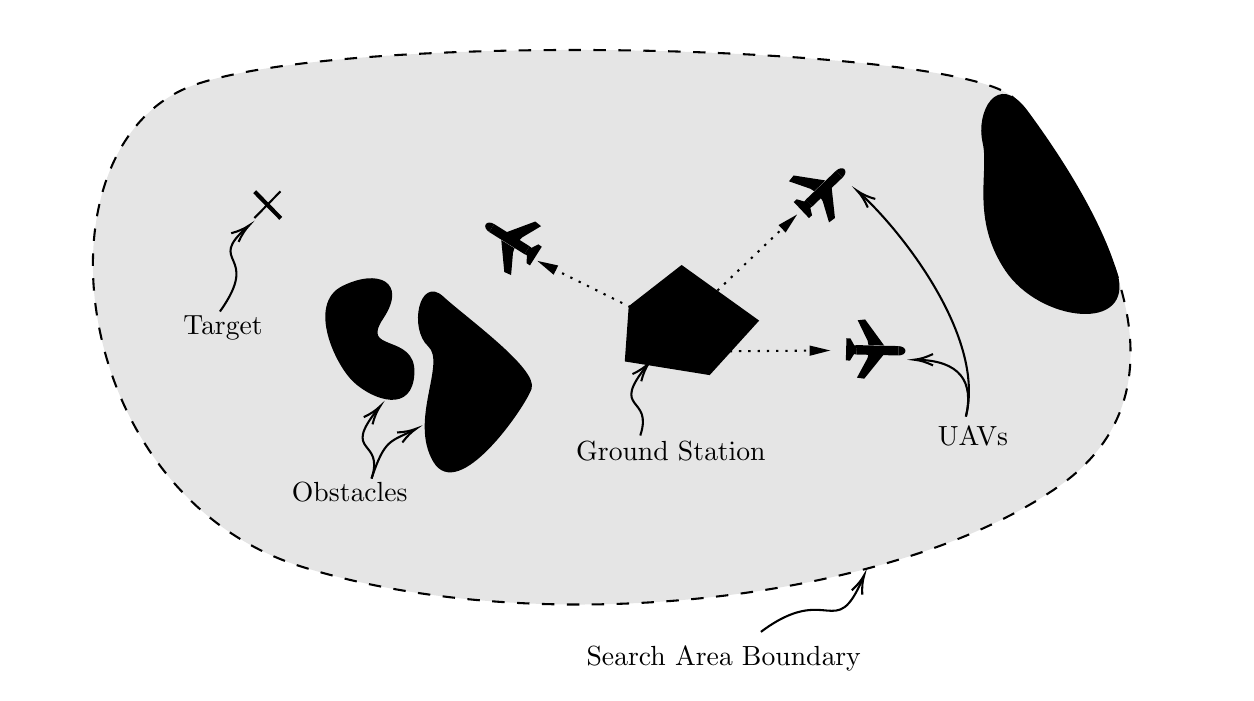
\begin{tikzpicture}[x=0.75pt,y=0.75pt,yscale=-0.83,xscale=0.83]
		%uncomment if require: \path (0,400); %set diagram left start at 0, and has height of 400
		
		%Straight Lines [id:da49540684334953466] 
		\draw  [dash pattern={on 0.84pt off 2.51pt}]  (331,163) -- (269.08,132.25) ;
		\draw [shift={(267.29,131.36)}, rotate = 386.40999999999997] [fill={rgb, 255:red, 0; green, 0; blue, 0 }  ][line width=0.08]  [draw opacity=0] (12,-3) -- (0,0) -- (12,3) -- cycle    ;
		%Straight Lines [id:da30158413299148346] 
		\draw  [dash pattern={on 0.84pt off 2.51pt}]  (364,156) -- (416.55,105.81) ;
		\draw [shift={(418,104.43)}, rotate = 496.32] [fill={rgb, 255:red, 0; green, 0; blue, 0 }  ][line width=0.08]  [draw opacity=0] (12,-3) -- (0,0) -- (12,3) -- cycle    ;
		%Straight Lines [id:da10124487148233396] 
		\draw  [dash pattern={on 0.84pt off 2.51pt}]  (352,184) -- (435.29,183.37) ;
		\draw [shift={(437.29,183.36)}, rotate = 539.5699999999999] [fill={rgb, 255:red, 0; green, 0; blue, 0 }  ][line width=0.08]  [draw opacity=0] (12,-3) -- (0,0) -- (12,3) -- cycle    ;
		%Shape: Chord [id:dp6980228508589381] 
		\draw  [draw opacity=0][fill={rgb, 255:red, 0; green, 0; blue, 0 }  ,fill opacity=1 ][line width=0.75]  (476.89,180.81) .. controls (476.89,180.81) and (476.89,180.81) .. (476.89,180.81) .. controls (479.16,180.86) and (480.98,182.12) .. (480.95,183.62) .. controls (480.92,185.13) and (479.05,186.3) .. (476.78,186.25) -- cycle ;
		%Shape: Rectangle [id:dp12203216080380419] 
		\draw  [draw opacity=0][fill={rgb, 255:red, 0; green, 0; blue, 0 }  ,fill opacity=1 ][line width=0.75]  (476.78,186.25) -- (452.58,185.69) -- (452.69,180.23) -- (476.89,180.79) -- cycle ;
		%Shape: Chord [id:dp22975070372280104] 
		\draw  [draw opacity=0][fill={rgb, 255:red, 0; green, 0; blue, 0 }  ,fill opacity=1 ][line width=0.75]  (452.58,185.69) .. controls (452.58,185.69) and (452.58,185.69) .. (452.58,185.69) .. controls (452.58,185.69) and (452.58,185.69) .. (452.58,185.69) .. controls (450.31,185.63) and (448.49,184.37) .. (448.52,182.87) .. controls (448.55,181.37) and (450.42,180.2) .. (452.69,180.25) -- cycle ;
		%Shape: Boxed Polygon [id:dp8761597599980013] 
		\draw  [draw opacity=0][fill={rgb, 255:red, 0; green, 0; blue, 0 }  ,fill opacity=1 ][line width=0.75]  (452.78,199.11) -- (458.9,187.83) -- (459.45,185.47) -- (468.38,185.63) -- (457.02,199.73) -- cycle ;
		%Shape: Boxed Polygon [id:dp5791137585698698] 
		\draw  [draw opacity=0][fill={rgb, 255:red, 0; green, 0; blue, 0 }  ,fill opacity=1 ][line width=0.75]  (453.21,165.81) -- (458.98,177.73) -- (459.45,180.19) -- (468.49,180.36) -- (457.52,165.33) -- cycle ;
		%Shape: Boxed Polygon [id:dp9103688732740809] 
		\draw  [draw opacity=0][fill={rgb, 255:red, 0; green, 0; blue, 0 }  ,fill opacity=1 ][line width=0.75]  (448.73,189.23) -- (446.33,189.08) -- (446.68,176.24) -- (448.99,176.34) -- (452.64,182.97) -- cycle ;
		
		%Shape: Chord [id:dp7068810176518192] 
		\draw  [draw opacity=0][fill={rgb, 255:red, 0; green, 0; blue, 0 }  ,fill opacity=1 ][line width=0.75]  (440.67,79.02) .. controls (442.31,77.45) and (444.49,77.05) .. (445.53,78.14) .. controls (446.57,79.22) and (446.08,81.37) .. (444.43,82.94) -- cycle ;
		%Shape: Rectangle [id:dp848693154857034] 
		\draw  [draw opacity=0][fill={rgb, 255:red, 0; green, 0; blue, 0 }  ,fill opacity=1 ][line width=0.75]  (444.43,82.94) -- (426.93,99.65) -- (423.14,95.71) -- (440.65,79) -- cycle ;
		%Shape: Chord [id:dp21428517784535273] 
		\draw  [draw opacity=0][fill={rgb, 255:red, 0; green, 0; blue, 0 }  ,fill opacity=1 ][line width=0.75]  (426.93,99.65) .. controls (426.93,99.65) and (426.93,99.65) .. (426.93,99.65) .. controls (426.93,99.65) and (426.93,99.65) .. (426.93,99.65) .. controls (425.29,101.22) and (423.11,101.62) .. (422.07,100.53) .. controls (421.03,99.45) and (421.52,97.3) .. (423.16,95.73) -- cycle ;
		%Shape: Boxed Polygon [id:dp15973791828664186] 
		\draw  [draw opacity=0][fill={rgb, 255:red, 0; green, 0; blue, 0 }  ,fill opacity=1 ][line width=0.75]  (436.56,109.01) -- (432.91,96.7) -- (431.63,94.64) -- (438.06,88.44) -- (440,106.44) -- cycle ;
		%Shape: Boxed Polygon [id:dp49966172959496835] 
		\draw  [draw opacity=0][fill={rgb, 255:red, 0; green, 0; blue, 0 }  ,fill opacity=1 ][line width=0.75]  (413.32,85.15) -- (425.83,89.5) -- (427.9,90.91) -- (434.41,84.63) -- (416.03,81.77) -- cycle ;
		%Shape: Boxed Polygon [id:dp787624194601164] 
		\draw  [draw opacity=0][fill={rgb, 255:red, 0; green, 0; blue, 0 }  ,fill opacity=1 ][line width=0.75]  (426.71,104.88) -- (424.9,106.47) -- (416.08,97.15) -- (417.78,95.58) -- (425.04,97.69) -- cycle ;
		
		%Shape: Chord [id:dp8227224522684633] 
		\draw  [draw opacity=0][fill={rgb, 255:red, 0; green, 0; blue, 0 }  ,fill opacity=1 ][line width=0.75]  (239.32,114.59) .. controls (239.32,114.59) and (239.32,114.59) .. (239.32,114.59) .. controls (237.4,113.39) and (236.48,111.37) .. (237.27,110.1) .. controls (238.07,108.82) and (240.27,108.77) .. (242.2,109.97) -- cycle ;
		%Shape: Rectangle [id:dp5534326460299863] 
		\draw  [draw opacity=0][fill={rgb, 255:red, 0; green, 0; blue, 0 }  ,fill opacity=1 ][line width=0.75]  (242.2,109.97) -- (262.71,122.82) -- (259.82,127.46) -- (239.31,114.61) -- cycle ;
		%Shape: Chord [id:dp4614178134059348] 
		\draw  [draw opacity=0][fill={rgb, 255:red, 0; green, 0; blue, 0 }  ,fill opacity=1 ][line width=0.75]  (262.71,122.82) .. controls (262.71,122.82) and (262.71,122.82) .. (262.71,122.82) .. controls (262.71,122.82) and (262.71,122.82) .. (262.71,122.82) .. controls (264.63,124.03) and (265.55,126.04) .. (264.76,127.32) .. controls (263.96,128.59) and (261.76,128.65) .. (259.83,127.44) .. controls (259.83,127.44) and (259.83,127.44) .. (259.83,127.44) -- cycle ;
		%Shape: Boxed Polygon [id:dp23919758506014732] 
		\draw  [draw opacity=0][fill={rgb, 255:red, 0; green, 0; blue, 0 }  ,fill opacity=1 ][line width=0.75]  (269.4,111.18) -- (258.37,117.76) -- (256.69,119.5) -- (249.1,114.79) -- (266.07,108.48) -- cycle ;
		%Shape: Boxed Polygon [id:dp3587634642403712] 
		\draw  [draw opacity=0][fill={rgb, 255:red, 0; green, 0; blue, 0 }  ,fill opacity=1 ][line width=0.75]  (252.01,139.58) -- (253.14,126.39) -- (253.99,124.03) -- (246.31,119.27) -- (248.06,137.79) -- cycle ;
		%Shape: Boxed Polygon [id:dp5249659868713439] 
		\draw  [draw opacity=0][fill={rgb, 255:red, 0; green, 0; blue, 0 }  ,fill opacity=1 ][line width=0.75]  (267.83,121.75) -- (269.82,123.11) -- (262.95,133.96) -- (261.02,132.69) -- (261.27,125.13) -- cycle ;
		
		%Shape: Polygon Curved [id:ds4256439449283196] 
		\draw  [color={rgb, 255:red, 0; green, 0; blue, 0 }  ,draw opacity=1 ][fill={rgb, 255:red, 0; green, 0; blue, 0 }  ,fill opacity=1 ] (154.29,146.5) .. controls (174.29,136.5) and (191.29,143.5) .. (177.29,164.5) .. controls (163.29,185.5) and (196.29,173.5) .. (195.29,196.5) .. controls (194.29,219.5) and (172.29,211.5) .. (161.29,201.5) .. controls (150.29,191.5) and (134.29,156.5) .. (154.29,146.5) -- cycle ;
		%Shape: Polygon Curved [id:ds33622105589259155] 
		\draw  [fill={rgb, 255:red, 0; green, 0; blue, 0 }  ,fill opacity=1 ] (526.29,62.5) .. controls (522.29,45.5) and (534.29,21.5) .. (551.29,44.5) .. controls (568.29,67.5) and (593,104.57) .. (603.29,138.5) .. controls (613.57,172.43) and (559.29,166.5) .. (539.29,136.5) .. controls (519.29,106.5) and (530.29,79.5) .. (526.29,62.5) -- cycle ;
		%Shape: Polygon Curved [id:ds8239570744541536] 
		\draw  [color={rgb, 255:red, 0; green, 0; blue, 0 }  ,draw opacity=1 ][fill={rgb, 255:red, 0; green, 0; blue, 0 }  ,fill opacity=1 ] (212.29,152.5) .. controls (225.29,164.5) and (267.29,194.5) .. (263.29,205.5) .. controls (259.29,216.5) and (221.29,271.5) .. (207.29,247.5) .. controls (193.29,223.5) and (215.29,190.5) .. (204.29,180.5) .. controls (193.29,170.5) and (199.29,140.5) .. (212.29,152.5) -- cycle ;
		%Shape: Polygon [id:ds8552542170764239] 
		\draw  [draw opacity=0][fill={rgb, 255:red, 0; green, 0; blue, 0 }  ,fill opacity=1 ] (351,133.71) -- (396,166) -- (367.29,197.64) -- (318,189.71) -- (320.29,157.64) -- cycle ;
		%Shape: Polygon Curved [id:ds09031265756878826] 
		\draw  [fill={rgb, 255:red, 0; green, 0; blue, 0 }  ,fill opacity=0.1 ][dash pattern={on 4.5pt off 4.5pt}] (70,28.57) .. controls (168,-3.43) and (519,6.57) .. (544.29,37.5) .. controls (569.57,68.43) and (666.29,195.64) .. (569.29,262.64) .. controls (472.29,329.64) and (267,351.71) .. (130,308.71) .. controls (-7,265.71) and (-28,60.57) .. (70,28.57) -- cycle ;
		%Straight Lines [id:da356677833966234] 
		\draw [line width=1.5]    (103.15,91.15) -- (118.29,106.64) ;
		%Shape: Boxed Line [id:dp01411653116334799] 
		\draw    (118.13,91) -- (103,106.49) ;
		
		%Curve Lines [id:da28671101836816915] 
		\draw    (327,232.71) .. controls (334.88,209.07) and (308.8,219.39) .. (330.95,191.99) ;
		\draw [shift={(332,190.71)}, rotate = 489.61] [color={rgb, 255:red, 0; green, 0; blue, 0 }  ][line width=0.75]    (10.93,-3.29) .. controls (6.95,-1.4) and (3.31,-0.3) .. (0,0) .. controls (3.31,0.3) and (6.95,1.4) .. (10.93,3.29)   ;
		%Curve Lines [id:da563480141441292] 
		\draw    (516,221.71) .. controls (520.87,201.24) and (512.44,189.32) .. (487.92,188.74) ;
		\draw [shift={(486,188.71)}, rotate = 360] [color={rgb, 255:red, 0; green, 0; blue, 0 }  ][line width=0.75]    (10.93,-3.29) .. controls (6.95,-1.4) and (3.31,-0.3) .. (0,0) .. controls (3.31,0.3) and (6.95,1.4) .. (10.93,3.29)   ;
		%Curve Lines [id:da18971834863536863] 
		\draw    (397,346.71) .. controls (436.4,317.16) and (439.9,353.59) .. (456.24,315.51) ;
		\draw [shift={(457,313.71)}, rotate = 472.52] [color={rgb, 255:red, 0; green, 0; blue, 0 }  ][line width=0.75]    (10.93,-3.29) .. controls (6.95,-1.4) and (3.31,-0.3) .. (0,0) .. controls (3.31,0.3) and (6.95,1.4) .. (10.93,3.29)   ;
		%Curve Lines [id:da6745919416459623] 
		\draw    (516,221.71) .. controls (527.76,175.65) and (478.05,113.27) .. (454.41,91.97) ;
		\draw [shift={(453,90.71)}, rotate = 401.01] [color={rgb, 255:red, 0; green, 0; blue, 0 }  ][line width=0.75]    (10.93,-3.29) .. controls (6.95,-1.4) and (3.31,-0.3) .. (0,0) .. controls (3.31,0.3) and (6.95,1.4) .. (10.93,3.29)   ;
		%Curve Lines [id:da25251752585399045] 
		\draw    (83,160.71) .. controls (107.62,126.24) and (74.04,133.48) .. (98.83,111.73) ;
		\draw [shift={(100,110.71)}, rotate = 499.57] [color={rgb, 255:red, 0; green, 0; blue, 0 }  ][line width=0.75]    (10.93,-3.29) .. controls (6.95,-1.4) and (3.31,-0.3) .. (0,0) .. controls (3.31,0.3) and (6.95,1.4) .. (10.93,3.29)   ;
		%Curve Lines [id:da20768778914859998] 
		\draw    (171,257.71) .. controls (178.88,234.07) and (152.8,244.39) .. (174.95,216.99) ;
		\draw [shift={(176,215.71)}, rotate = 489.61] [color={rgb, 255:red, 0; green, 0; blue, 0 }  ][line width=0.75]    (10.93,-3.29) .. controls (6.95,-1.4) and (3.31,-0.3) .. (0,0) .. controls (3.31,0.3) and (6.95,1.4) .. (10.93,3.29)   ;
		%Curve Lines [id:da8608303007049891] 
		\draw    (171,257.71) .. controls (178.68,234.67) and (181.75,236.52) .. (195.26,229.62) ;
		\draw [shift={(197,228.71)}, rotate = 511.93] [color={rgb, 255:red, 0; green, 0; blue, 0 }  ][line width=0.75]    (10.93,-3.29) .. controls (6.95,-1.4) and (3.31,-0.3) .. (0,0) .. controls (3.31,0.3) and (6.95,1.4) .. (10.93,3.29)   ;
		
		% Text Node
		\draw (288,234) node [anchor=north west][inner sep=0.75pt]   [align=left] {Ground Station};
		% Text Node
		\draw (498,226) node [anchor=north west][inner sep=0.75pt]   [align=left] {UAVs};
		% Text Node
		\draw (294,353) node [anchor=north west][inner sep=0.75pt]   [align=left] {Search Area Boundary};
		% Text Node
		\draw (60,161) node [anchor=north west][inner sep=0.75pt]   [align=left] {Target};
		% Text Node
		\draw (123,258) node [anchor=north west][inner sep=0.75pt]   [align=left] {Obstacles};
		
		
	\end{tikzpicture}

	\caption{Diagram showing the general components of a Search and Rescue problem with multiple UAVs.}
	\label{fig:CM01}
\end{figure}
\section{Search Area}
\label{sec:CM Search-Area}
\acf{sar} is generally classified according to the terrain, seen as this would determine what type equipment, personnel and vehicles may be required. In general, \ac{sar} is divided into ground, urban, mountain, cave, combat or maritime rescue \cite{Leis2021}.

Ground or lowland \ac{sar} refers to any mission carried out on land. The rescue team generally consists of people on foot. This can include plains, dense forests and other wilderness regions. Urban rescue is often preceded by a disaster that causes an urban area to become treacherous. An earthquake or explosion may cause building collapses that may require this type of rescue. 

Mountain and cave rescue are often grouped together. However, aerial support in the case of cave rescues is not very useful, and so it is separated out for the purpose of this paper. Mountain rescue generally refers to situations where people become lost or trapped in mountainous regions. This often includes terrain that is difficult to traverse, such as shear cliff faces.

Combat rescue refers to any rescue carried out in a war-like context. This type of rescue will not be addressed in detail in this paper, seen as the circumstances of a battlefield are volatile and unpredictable compared to the other scenarios, and would require unique consideration.

Lastly, maritime search and rescue concerns rescue within the context of some body of water. This could include people who are victims of a sunken boat or perhaps a crashed aircraft. People who get swept up from the coast by rip currents would also be in this category. 

The extent of assistance that automated \acp{uav} can provide would depend on the type of rescue. In wide open plains or oceans with few obstructions, they would have a clear view of the search area from any visual or thermal camera. In densely forested areas, visibility may be limited and aerial support would be unhelpful. In a mountainous region where the altitudes are too high or the temperatures are too low for a \ac{uav} to sustain flight they can also not be used. 

Unfavourable weather conditions would also have a large impact. High wind speeds could make it impossible to fly, and heavy rains or fog may make visibility very low. Moreover, at night \acp{uav} may have to rely on thermal images, due to lack of visibility with a conventional camera.

In general \acp{uav} suffer from similar limitations that manned aircraft would, and it is assumed that they would be used with the same discretion. One advantage is that if a \ac{uav} flies in dangerous conditions, no pilot is placed in danger and the worst case scenario involves a crashed \ac{uav}.

If an area can benefit from an aerial search using \acp{uav}, it is assumed they would be expected to assist the search of a bounded geographical region. % How are search regions generally defined 

The environment wherein the \acp{uav} are expected to assist the search operation is a bounded region. Every point within the environment map should be reachable from any other point in the map.

Obstacles in the environment could represent any region wherein the \acp{uav} must not fly. This could be a no-fly zone or a physical obstruction at the \ac{uav}'s altitude. A section wherein it would not be beneficial to use a \ac{uav} to search for a target, such as a densely forested region, can be seen as an obstruction. A mountainous region where the altitudes are to high to fly a \ac{uav} can be an obstruction as well, or perhaps a region of bad weather conditions. 

It is the responsibility of the search team to mark out these obstructions and no-fly areas so they can be excluded from the search. A dynamic environment with moving obstacles is not modelled. It is reasonable to assume that \acp{uav} fly at a high enough altitude that no dynamic obstacles need to be modelled. The entire environment can be known prior to \ac{uav} flight, and all obstacles within it are static.
% TODO: elaborate on why this is a valid assumption.  
\section{Environment Model}

\section{UAV Model}
% TODO: "A constant altitude above the surface of the ground or ocean is assumed to be maintained in order to achieve a constant \ac{fov}." - not sure if this complicates the calculations
\section{Collision Model}

\section{Target Model}
In the context of \ac{sar}, a target is generally a victim that requires rescue. This may be anyone that is in some form of peril within a terrain, that requires assistance.

The target is assumed to be static within the environment. This is a valid assumption in the event that someone is trapped in difficult terrain or is injured and cannot move, which are often the case in a rescue operation. Victims are also often advised to stay put when awaiting a search team, and it is therefore assumed that in most scenarios they would.

There may be some situations wherein the target is in motion, but is lost within some terrain. However, accounting for a target in motion requires predicting their motion, or using data to estimate target trajectory as the search progresses. This is often very intuitive and may be best if left to an experienced conventional rescue team. 

An approach where the target is assumed to be static may still achieve success even though the target is dynamic, which means that it could still assist in a rescue operation with a dynamic target. For example, if a sweep of the environment is used, and does not initially locate a dynamic target, the sweep can simply be performed multiple times, but this is quite sub-optimal.
% TODO: cite something to back this up
\section{Target Detection}
% Assume static target
% Assume the use of a visual or thermal camera
% FOV calculations
% Assume target is detected when in FOV  - either by human observers or image recognition (there might be a communications delay, but this is assumed to be negligible)
For the purpose of this paper it is assumed that the \acp{uav} have on-board cameras. These could be thermal or visual cameras, or both. Historically, these have been used in tandem for target detection from a \ac{uav}. Section \ref{} discusses an implementation where a thermal camera is used to find potential victims and a visual camera is used to verify \cite{}. 

In general, the consensus for \ac{sar} is that a false positive detection is acceptable, but a failed detection is not \cite{}. This is assumed to be the bias of the algorithm that will be used, and it is therefore it is assumed that a target will always be detected when in view. 
% What happens in the case of a false positive

Target detection can be online or offline. The processing can be done on-board the \ac{uav}, but this means that the \ac{uav} may require more processing power and as a result have heavier, more expensive equipment on-board. It is therefore favourable to have this processing done in post at a ground station. This requires a stable communication link. Real-time data transfer would be ideal.
% Mention that application with the uav formation flying to achieve a stable link - this can be done when a target is detected. For the purpose of this

Data delays are common, but it is assumed that these delays are negligible and would not noticeably affect the time to find a target. Therefore, the assumption is that real-time data transfer is achieved. Communication failures can also negatively influence the performance of \acp{uav} in assisting \ac{sar}. However, it is assumed that the \acp{uav} would store enough of the data captured on-board to ensure that it reaches the ground station once communication is re-established. 

This makes it favourable that the \acp{uav} can follow some planned path without contact with a ground station. It should either have a pre-planned path that it can navigate or some online mechanism to plan its own path during flight. A pre-planned path has the advantage of ensuring very little on-board processing is required, whereas the online approach may be more reactive ina  changing environment. It is intuitive to assume that an on-board GPS would help the \ac{uav} navigate along its path.

A manned aircraft does not rely on communication links to the same extent and can immediately execute a rescue if a target is found. However, if a target is not reachable via repelling, they would rely on communication with a ground team, just as a \ac{uav} would.

Generally manned vehicles rely on people on-board to spot the target, while the pilot flies. For \acp{uav}, the ground team would observe transmitted video footage in order to locate a target, whilst safely on the ground. Moreover, they could use target detection algorithms that process the images to detect targets and provide additional assistance. \acp{uav} that have a carrying capacity can also be used to deliver essential supplies to a victim as soon as they are located. Flying close to the ground or surface of water is a much less risky manoeuvre for an unmanned vehicle. 

Cameras can be placed on a gimble and it is therefore assumed that the camera angle can be adjusted to always point exactly downwards toward the ground or ocean. 

In summary, it is assumed that the target is static and will be detected when within the view of some visual or thermal camera on-board the \ac{uav}. It is important to clarify what it means to be within view. For the case of an on-board camera, this means the victim or target is detected the moment it enters the \ac{fov} of the camera. 

%TODO: Should this section be split in two and should the camera FOV calculation be included here


